\documentclass[11pt]{article}
\usepackage{graphicx}
\graphicspath{{./images/}} % tell it where to look for graphics
\usepackage[margin=0.75in]{geometry} % to set margins
\usepackage{setspace} % to set line spacing
\usepackage{parskip} % for proper paragraph spacing without indents
\usepackage{fontspec} % for setting fonts
\setlength{\parindent}{0cm} % set no ident between paragraphs
\setmainfont{Palatino Linotype} % set the font
\renewcommand{\contentsname}{Table of Contents} % change default name of table of contents
\begin{document}
\begin{titlepage}

\newcommand{\HRule}{\rule{\linewidth}{0.5mm}}

\begin{center}

% Upper part of the page
%
\includegraphics[width=0.15\textwidth]{./logo}\\[1cm]    

% Company Name
\textsc{\LARGE Tau Labs}\\[1.5cm]

% Document Type
\textsc{\Large Software Development Agreement}\\[1.5cm]

% Document Title
\HRule \\[0.4cm]
{ \huge \bf Snopsize}\\[0.4cm]
\HRule \\[1.5cm]

% Author and supervisor
\begin{minipage}{0.4\textwidth}
\begin{flushleft} \large
\emph{Created By:}\\
Ian \textsc{Clarkson} \\
Dinko \textsc{Harbinja} 
\end{flushleft}
\end{minipage}

\vfill

% Bottom of the page
{\large \today}

\end{center}

\end{titlepage}
\newpage
%\tableofcontents % optional table of contents -- not necessary for a legal document
\newpage
\section*{}
\begin{center}
{\bf \LARGE Software Development Agreement} 
\end{center}
\setlength{\parskip}{24pt} % set spacing between paragraphs
This Software Development Agreement (the "Agreement") is effective upon date of signature.
\setlength{\parskip}{6pt} % set spacing between paragraphs
\begin{tabbing}
{\bf BETWEEN}:\hspace{0.2in}\={\bf Eoin Corrigan} (the "Customer") \\
\> \\
{\bf AND}:\> {\bf Tau Labs } (the "Developer"), a partnership organized and existing under the laws \\
\>of the Province of Ontario, with its head office located at: \\
\> \\
\>212-51 Saddlecreek Dr. \\
\> Markham, Ontario,  L3T 7Z1 \\
\end{tabbing}
The Customer and Developer agree as follows:
\section{Motivation}
snopsize.com is envisioned as a web application to assist in the creation and sharing of succinct, structured information. It asks its users to distill disparate sources of data to their fundamental essence. The larger community may then examine and share this information, not only for the purpose of discovering new facts and ideas, but also to help commit existing ones to memory. Users will be drawn to snopsize.com for the ease with which it allows them to summarize various media into a standard, digestible template suitable for sharing with others.
\section{Purpose of Agreement}
Customer desires to retain Developer as an independent contractor to develop the computer software (the "Software") described in the Functional Specifications (the "Specifications") (see section \ref{sec:functional_spec}) of this Agreement. Developer is ready, willing, and able to undertake the development of the Software and agrees to do so under the terms and conditions set forth in this Agreement.
\section{Functional Specification}
\label{sec:functional_spec}
\subsection{Introduction}
Four operations are seen as being critical to the foundation of snopsize.com: Create, Search, Save, and Browse. The Create operation is the ability to create a new snop. All registered users will have this ability. Search is the ability to sift through all submitted snops to locate ones of interest. Search may be based on keyword, user name, or source URL. Save implies the ability to mark other users' snops as being of particular interest. Saved snops will remain available to a user. Browse is the ability to peruse sets of related snops. Snops may be related because they were written by the same user, related to the same source URL, or related in some other fashion entirely.
\subsection{Snop Definition and Structure}
\label{sec:snop_structure}
A "snop" is a self-contained collection of facts or points drawn or deduced from a particular source. This source may be a news article or a book, but the concept of a snop itself is not limited to any particular media. Central to the approach of snopsize.com is a common template for all snops. A snop will consist of the following fields:
\begin{enumerate}
\item User (Mandatory)
\item Title (Mandatory)
\item Source URL (Optional)
\item Point 1 (Optional)
\item Point 2 (Optional)
\item Point 3 (Optional)
\item Summary (Optional)
\end{enumerate}
Any fields marked as optional may be left empty during the creation of a new snop. This allows for some flexibility when summarizing more simplistic sources, but limits the upper complexity of a snop to a manageable chunk. The snop structure consists of three main points. This forms an essay-style structure in which there is a title, three points, and a summary.
\subsection{Home Page}
\begin{figure}[htb]
\begin{center}
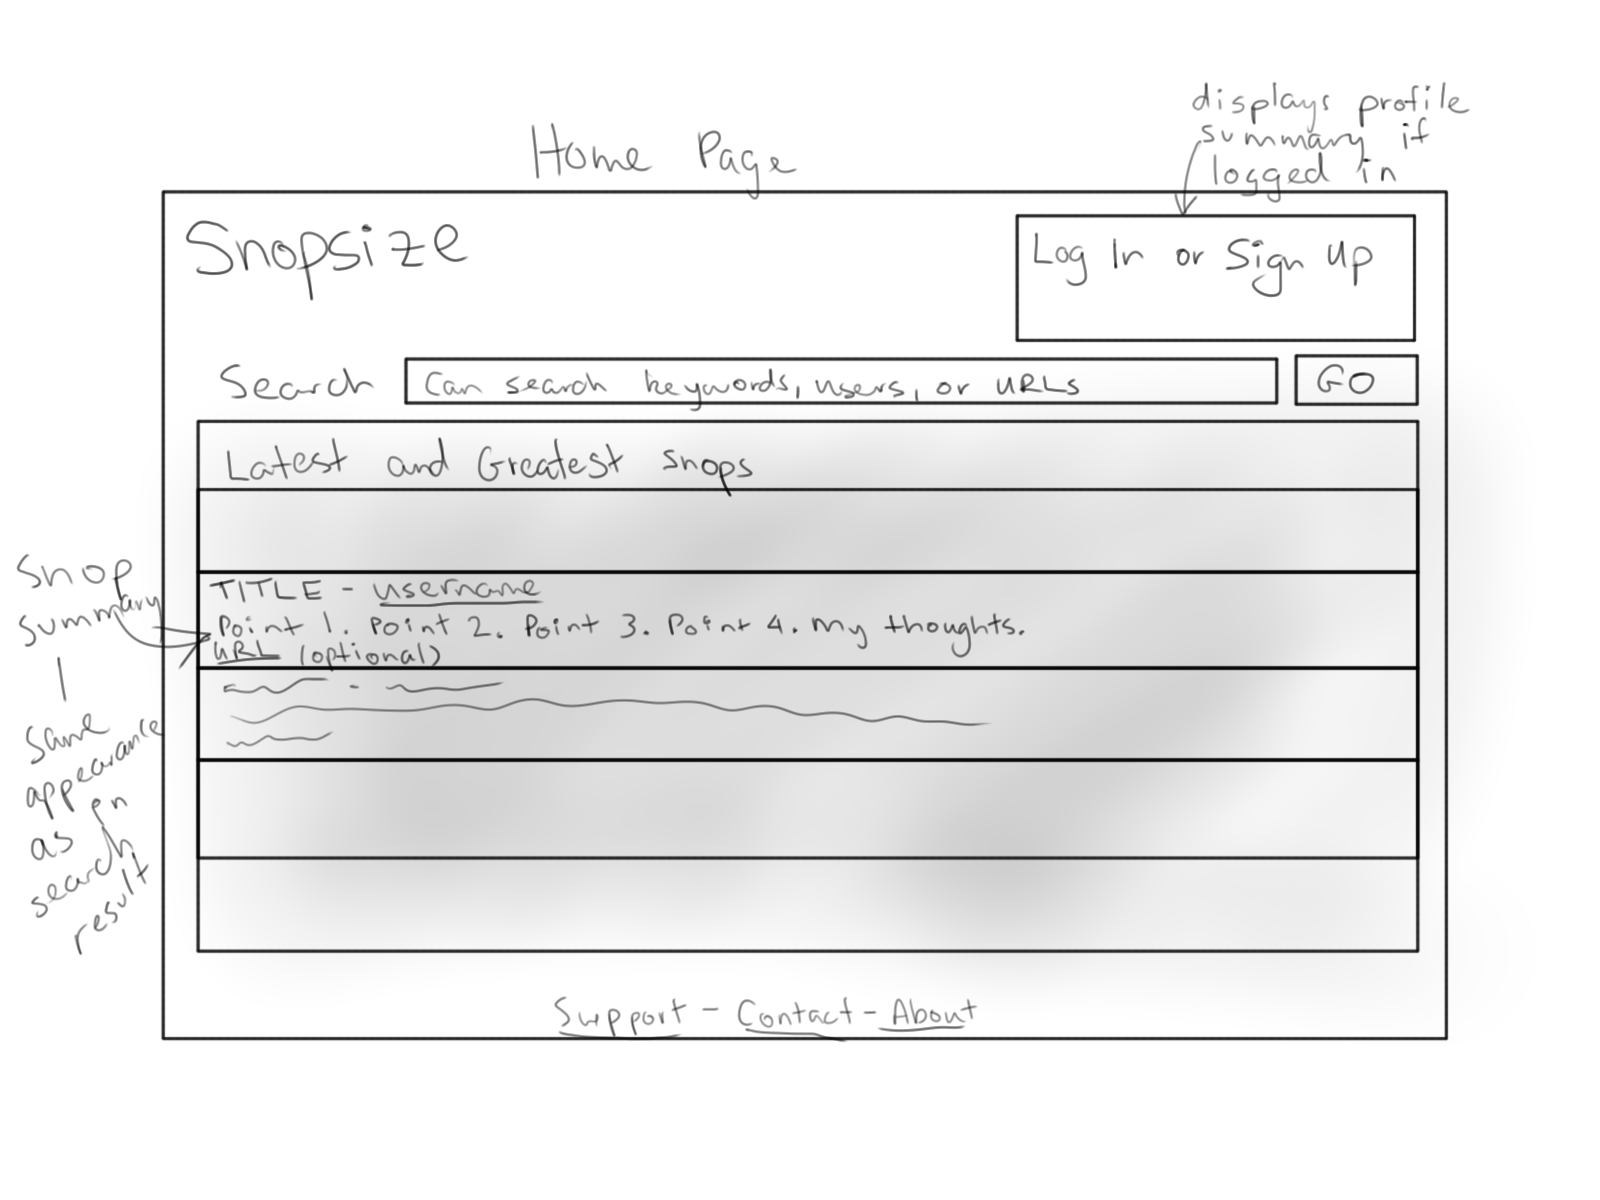
\includegraphics[width=0.9\textwidth]{home_page.png}
\caption{Home Page}
\label{fig:fig_home_page}
\end{center}
\end{figure}
The Home Page is the page a user will first encounter upon visiting snopsize.com. A list of "top" snops will appear on this page. These will be the most recent snops, snops that have been saved frequently (popular snops), or a combination of both.

Links will be available within each snop to navigate to all of the snops from the author of the given snop, and also to all snops related to the same source URL.

A user will have the ability to search for snops from this page. For more detail on search functionality, please reference section \ref{sec:search_results_page}. 

If users are not logged in, they will have the option to either log in with their existing account, or to create an account if they do not have one. If users have forgotten their password they will have the ability to reset their password via an email link.

If the user is already logged in they will have the ability to log out, as well as access their User Page (see section \ref{sec:user_page}). 

General site navigation will be available at the bottom of the page and will be common to all pages on snopsize.com. This area may include links such as "About", "Contact", and "Site Map".
\subsection{Sign Up Page}
This is the page that is shown to a new user who wishes to sign up. It should be directly accessible from most areas of the site. Many features of the site will operate properly without a user being signed up. However, saving snops from other users and creating new snops will both require a user account. A single user name should be linked to a specific email address. No more than one user name should be allowable per email address. Sign up should also require a certain password strength. Forgotten login credentials may be dealt with using password reset emails.
\subsection{Snop View}
Snops must be viewable in multiple perspectives. A Search Result (see section \ref{sec:search_results_page}) containing snops can't visually display them in their entirety. As such, snops will need a short line item view which contains an overview or snapshot of the snop content. A full snop view is also necessary for a user to see the entirety of a snop at once. This view will be used on the Related Page (see section \ref{sec:related_page}) and the User Page (see section \ref{sec:user_page}) to show the snop contents. 

Both the full snop view and the line item snop view should have user- and URL-based links. From a snop, a user should be able to quickly navigate to related snops or to other snops written by the same user. The full snop view should also have the ability to save a snop to a user's snops if the snop was not written by that user. This feature will also be possible directly from the line item view. It is presumed that at full size, only one snop is likely to be able to be shown at any given time on a given device.
\subsection{Search Results Page}
\label{sec:search_results_page}
\begin{figure}[htb]
\begin{center}
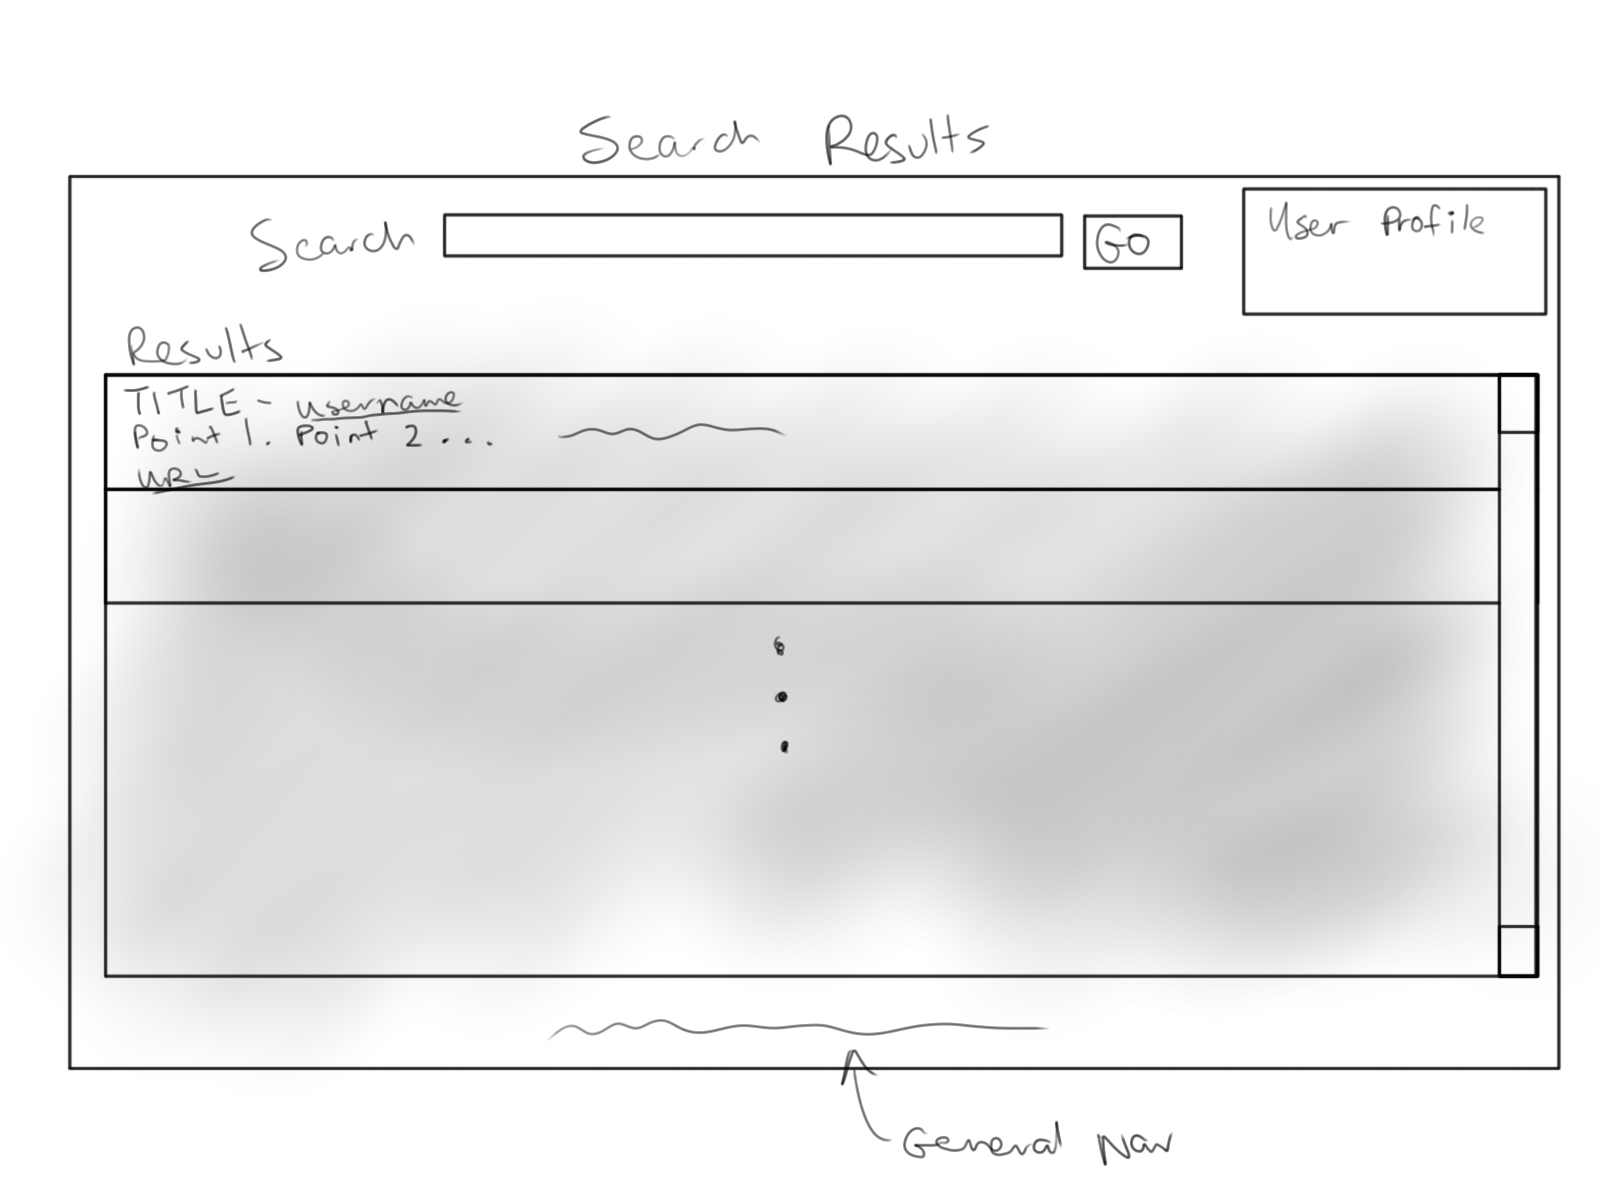
\includegraphics[width=0.9\textwidth]{search_results.png}
\caption{Search Results Page}
\label{fig:fig_search_results_page}
\end{center}
\end{figure}
The Search Page allows users to search for snops. A search will simultaneously examine three distinct areas: users, source URLs, and keywords.

A search term may be seeking a particular user name. In such a case, the search results should contain user names similar to the search query. The user would then be able to follow a link to the relevant User Page (see section \ref{sec:user_page}).

A search term may be seeking snops related to a particular source URL. If a direct match is made on the source URL, the search result will take you directly to the Related Page (see section \ref{sec:related_page}) for the given source URL. If no direct match is found, the site user will be told that the source URL is not found and will be given an option to create the first snop for that particular source URL.

Finally, a search term may be seeking snops related to a given keyword. In such a case, the search results should contain snops containing instances of those keywords. The snops would show up in a summary view so that the site user can quickly look through them.

A search result will contain two possible links to pursue the given snop. One link will be related to the user name of the creator of the snop. Following that link will lead to a display of all of that user's snops, with the linked snop shown full size. The site user may then choose to navigate to other snops created by the same user.

Alternatively, the site user may follow a link related to the source URL of the snop. Note that this will only be possible if the original snop contained a source URL. Following such a link, the site user will be presented with a list of snops related to the same source URL as the given snop. This dual-view approach to browsing snops will be common to other areas of the site.

The intention will be to simplify the Search function by not requiring a user to enter a search type (user, keyword, or URL). Developer may, however, find that a search type is required to narrow down search results.
\subsection{Related Page}
\label{sec:related_page}
The Related Page contains listings of snops that all reference the same source URL. All of the snops should be directly related in that they were written about the same original article or web page. Source URLs must match exactly to be linked in the Related Page. It will be possible to create a new snop regarding the particular source URL from this page. 
\subsection{User Page}
\label{sec:user_page}
\begin{figure}[htb]
\begin{center}
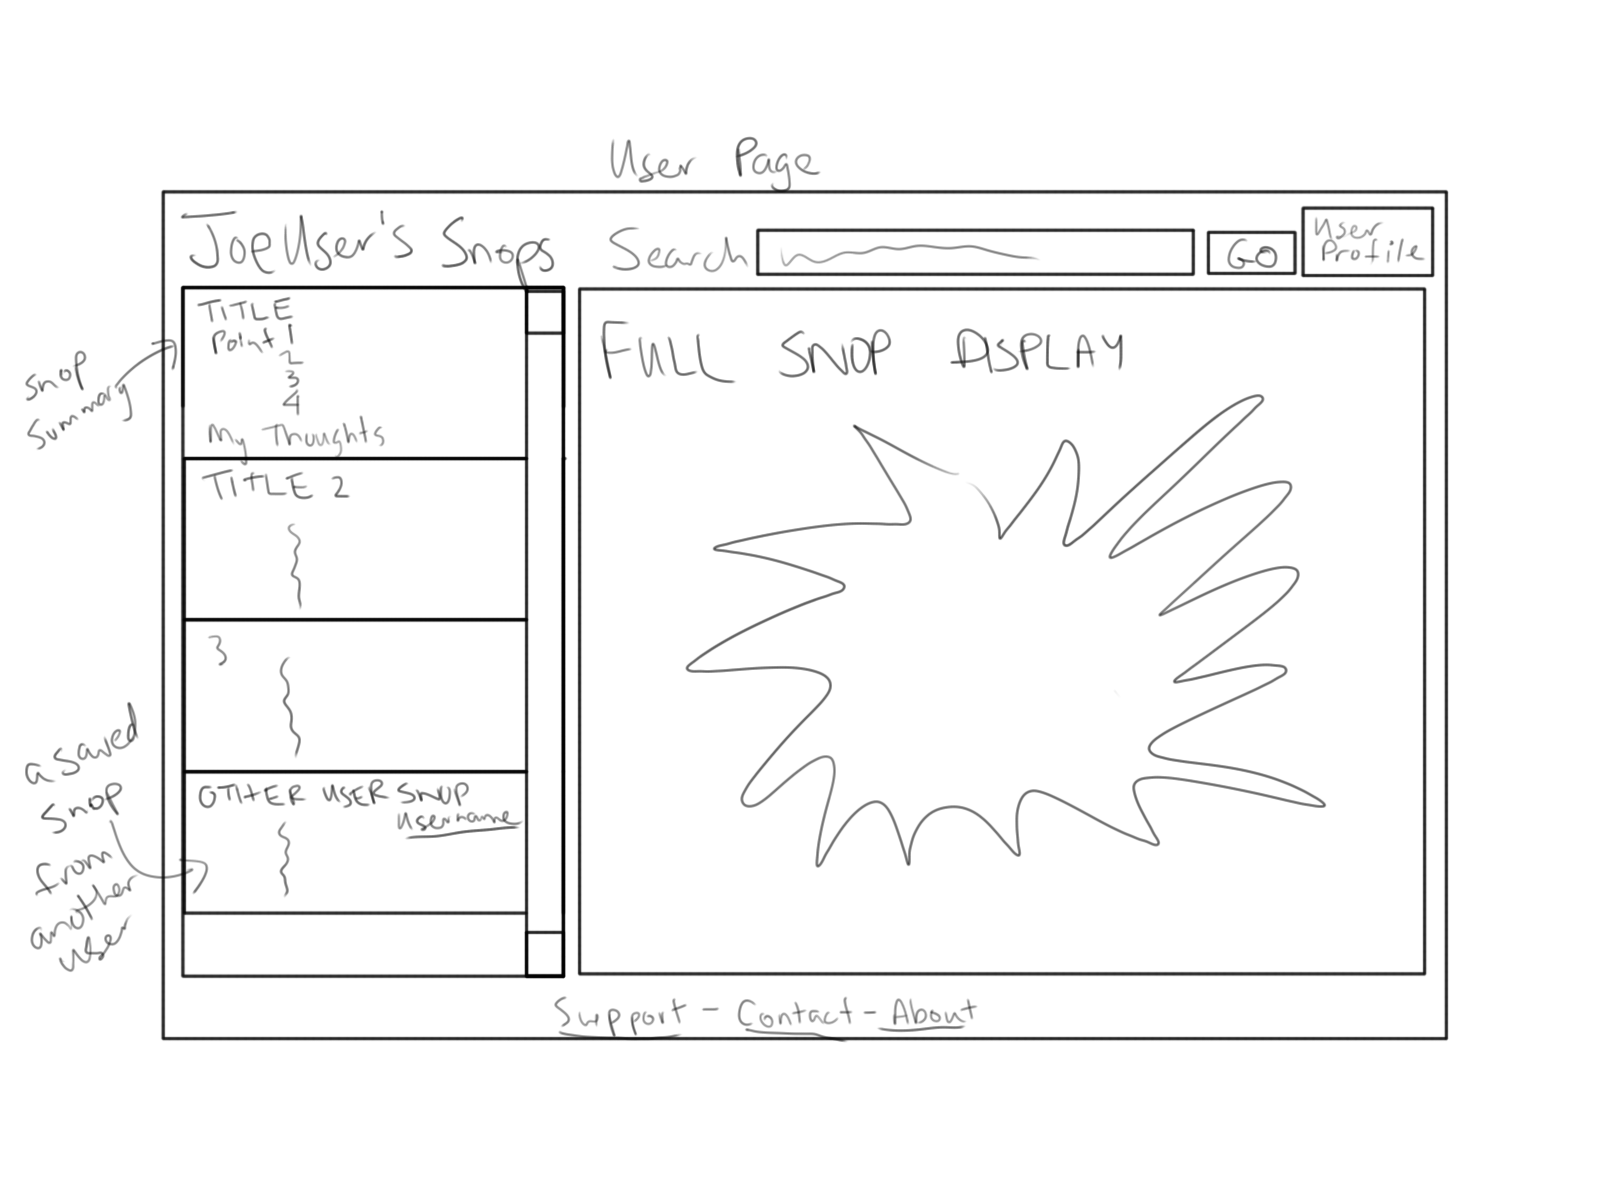
\includegraphics[width=0.9\textwidth]{user_page.png}
\caption{User Page}
\label{fig:fig_user_page}
\end{center}
\end{figure}
The User Page contains listings of snops that were created by a single user. The listing will also contain snops from other authors saved by the given user. The two types will be differentiated. 

All snops generated by a user will be made public. Snops will be uneditable once created. They may, however, be deleted. Inability to edit means that a user will never be surprised when a snop they saved changes. Ability to delete allows users who do not wish to share certain information to remove it. Any existing links to that snop will still function, but will produce a message that the given snop has been removed. 

If users are viewing their own User Page, they will also be able to create a new snop.
\subsection{Snop Creation Page}
The act of creating a snop will require its own interface. Users may enter information in any of the snop fields. The user can indicate completion through a "Snop" button. Only some snop fields will be considered mandatory (see section \ref{sec:snop_structure}). A snop must have a title and a user name. The user name will be guaranteed to be valid, since only users who have signed up for the service will be able to create snops. Snop titles are not required to be unique.

Initially, the snop boxes will all be shown but are blank. The user may move through the boxes in any order to insert the desired text before completing the snop. The snop creation process may be cancelled at any point during the creation. 

Behaviour upon completion of the snop should be context-sensitive. If the user initially created the snop from a Related Page, the user should be returned to that page and have their snop displayed. Likewise, if the user created the snop from their own User Page, they should be returned to that page and have their snop displayed.
\section{Non-Functional Requirements}
\subsection{Languages and Internationalization}
American English will be the only supported language in which to view the site. Snops themselves may be written in any language, but the site itself will not be translated into multiple languages.
\subsection{Software Requirements}
The web service will run correctly on the three top platforms (PC, Mac, and Linux). Across platforms, support is planned for the following browsers:
\begin{enumerate}
\item Chrome
\item Firefox
\item Internet Explorer
\item Safari
\end{enumerate}
Although every effort will be made to support legacy browsers, identical appearance and performance cannot be guaranteed in outdated versions of the browsers named above.
\subsection{Visual Design}
Visual design of the web application will be outsourced to a third party. Developer will require express approval from Customer regarding visual design of the web application. The costs incurred as a result of visual design will be the responsibility of the Developer.
\subsection{Web Hosting}
Customer will be responsible for hosting Software and paying any costs related to web hosting. Depending upon the technology chosen to develop Software, Developer may request Customer to switch hosting provider. This will ensure that Software executes properly and performs as expected. Any costs related to switching hosting arrangements will be paid for by Customer.
\subsection{Deployment}
Developer will be responsible for supervising initial Software deployment. Customer may be required to provide assistance or information pertaining to the deployment. Customer's assistance or information includes, but is not limited to:
\begin{enumerate}
\item Login information required to access the production server
\item Providing hardware to deploy Software
\item Any additional hardware or software requirements 
\end{enumerate}
\section{Delivery}
\subsection{Deliverables}
Developer will deliver Software which includes, but is not limited to:
\begin{enumerate}
\item Source code
\item Visual design assets 
\item Documentation
\end{enumerate}
\subsection{Schedule}
Developer will deliver Software to Customer within 8 weeks of the signing of this Agreement. 

Each week, Developer will provide Customer with an intermediate deliverable that shows the functionality of Software at that point in time. The intermediate deliverable may implement a subset of the deliverables specified above. 
\subsubsection{Delay}
Developer shall use all reasonable efforts to deliver Software on schedule. However, at its discretion, Developer can extend the due date for any deliverable by giving written notice to Customer. The total of all such extensions shall not exceed 15 days. 
\section{Payment}	
Customer will pay Developer a total of \$15,000 CAD for the development of the Software. \$5000 CAD shall be paid within one week of the acceptance of this agreement, and \$10,000 CAD shall be paid upon completion and delivery of Software. All aforementioned costs are inclusive of taxes.
\section{Payment of Developer's Costs}
Customer shall reimburse Developer for the cost of any development software or commercial software libraries the developer deems necessary to complete Software, subject to approval by Customer.
\section{Changes in Specifications}
Customer may, in its sole discretion, request that changes be made to the Specifications, or other aspects of the Agreement and tasks associated with this Agreement. If Customer requests such a change, Developer will use its best efforts to implement the requested change at no additional expense to Customer and without delaying delivery of Software. In the event that the proposed change will, in the reasonable opinion of Developer, require a delay in the delivery of Software or would result in additional expense to Customer, then Customer and Developer shall confer and Customer shall, in its discretion, elect either to withdraw its proposed change or require Developer to deliver the Software with the proposed change and subject to the delay and/or additional expense.
\section{Acceptance Testing of Software}
Customer shall have 15 days from the date of delivery of Software in final form to inspect, test and evaluate it to determine whether Software satisfies the functionality set forth in the Specifications.

If Software does not satisfy said functionality, Customer shall give Developer written notice stating why Software is unacceptable. Developer shall have 15 days from the receipt of such notice to correct the deficiencies. Customer shall then have 15 days to inspect, test and evaluate Software. If Software still does not satisfy the functionality set forth, Customer shall have the option of either (1) repeating the procedure set forth above, or (2) terminating this Agreement pursuant to section \ref{sec:termination}. If Customer does not give written notice to Developer within the initial 15 day inspection, testing and evaluation period or any extension of that period that Software does not satisfy the functionality, Customer shall be deemed to have accepted the Software upon expiration of such period.
\section{Ownership of Software}
Developer assigns to Customer its entire right, title and interest in anything created or developed by Developer for Customer under this Agreement ("Work Product") including all patents, copyrights, trade secrets and other proprietary rights. This assignment is conditioned upon full payment of the compensation due to Developer under this Agreement. 

Customer assigns Developer rights to make mention of Work Product for the purposes of marketing. This includes, but is not limited to, images of the Work Product, screenshots, and other media.
\section{Ownership of Background Technology}
Customer acknowledges that Developer owns or holds a license to use and sublicense various pre-existing development tools, routines, subroutines and other programs, data and materials that Developer may include in the Software developed under this Agreement. This material shall be referred to as "Background Technology."  

Developer retains all right, title and interest, including all copyright, patent rights and trade secret rights in the Background Technology. Subject to full payment of the consulting fees due under this Agreement, Developer grants Customer a nonexclusive, perpetual worldwide license to use Background Technology in Software developed for and delivered to Customer under this Agreement, and all updates and revisions thereto. However, Customer shall make no other commercial use of the Background Technology without Developer’s written consent.
\section{Warranty}
\begin{enumerate}
\renewcommand{\labelenumi}{(\Alph{enumi})}
\item {\bf Warranty of Software Performance}: Developer warrants that for 6 months following acceptance of the Software by Customer, Software will be free from reproducible programming errors and defects in workmanship, and will substantially conform to the Specifications when operated in accordance with Specifications. If reproducible programming errors are discovered during the warranty period, Developer shall promptly remedy them at no additional expense to Customer. This warranty to Customer shall be null and void if Customer is in default under this Agreement or if the non-conformance is due to:
\begin{itemize}
\item Hardware failures due to defects, power problems, environmental problems or any cause other than Software itself;
\item Modifications of Software operating systems or computer hardware by any party other than Developer; or
\item Misuse, errors or negligence of Customer, its employees or agents in operating Software. Developer shall not be obligated to cure any defect unless Customer notifies it of the existence and nature of such defect promptly upon discovery
\end{itemize}
\item {\bf  Warranty of Compatibility}: Developer warrants that Software shall be compatible with Customer's hardware and software as set forth in the Specifications. 
\end{enumerate}
The warranties set forth in this agreement are the only warranties granted by Developer. Developer disclaims all other warranties express or implied. This includes, but is not limited to, any implied warranties or merchantability or fitness for a particular purpose.
\section{Term of Agreement}
This Agreement shall commence upon date of signutare and continue until all of the obligations of the parties have been performed or until earlier terminated as provided herein.
\section{Termination of Agreement}
\label{sec:termination}
Each party shall have the right to terminate this Agreement by written notice to the other if a party has materially breached any obligation herein and such breach remains uncured for a period of 30 days after written notice of such breach is sent to the other party.
If Developer terminates this Agreement because of Customer's fault, all of the following shall apply:
\begin{enumerate} \itemsep0pt \parskip0pt \parsep0pt
\renewcommand{\labelenumi}{(\Alph{enumi})}
\item Customer shall immediately cease use of Software. 
\item Customer shall, within 10 days of such termination, deliver to Developer all copies and portions of the Software and related materials and documentation in its possession furnished by Developer under this Agreement. 
\item All amounts payable or accrued to Developer under this Agreement shall become immediately due and payable. 
\item All rights and licenses granted to Customer under this Agreement shall immediately terminate. 
\end{enumerate}
\section{Signatures}
Each party represents and warrants that on this date they are duly authorized to bind their respective principals by their signatures below.

In witness whereof, the parties have executed this Agreement on the dates set forth first above, with full knowledge of its content and significance and intending to be legally bound by the terms hereof.

% The signature lines and text
\setlength{\parskip}{20pt} % set spacing between paragraphs
\par\noindent\makebox[2.5in][l]{CUSTOMER}      \hfill\makebox[2.5in][l]{DEVELOPER}%
\setlength{\parskip}{15pt} % set spacing between paragraphs
\par\noindent\makebox[2.5in]{\hrulefill} \hfill\makebox[2.5in]{\hrulefill}%
\setlength{\parskip}{0pt} % set spacing between paragraphs
\par\noindent\makebox[2.5in][l]{Signature}      \hfill\makebox[2.5in][l]{Signature}%
\setlength{\parskip}{15pt} % set spacing between paragraphs
\par\noindent\makebox[2.5in]{\hrulefill} \hfill\makebox[2.5in]{\hrulefill}%
\setlength{\parskip}{0pt} % set spacing between paragraphs
\par\noindent\makebox[2.5in][l]{Date}      \hfill\makebox[2.5in][l]{Date}%

\end{document}
